\chapter{Introduction}
\label{Chapter-Introduction}
In recent years, edge devices with advanced computing and data collection capabilities are becoming commonplace. As a result, massive volumes of new and useful data are generated, which can be exploited in Machine Learning (ML). When combined with recent advances and techniques in ML, new opportunities emerge in a variety of fields, including self-driving automobiles and medical applications. 

Traditional ML approaches demand the data to be consolidated in a single entity where learning takes place. However, due to unacceptable latency and storage requirements of centralizing huge amounts of raw data, this may be undesirable. To address the inefficiency of data silos, cloud computing architectures such as Multi-access edge computing (MEC) \cite{MEC} have been proposed in order to transfer the learning closer to where the data is produced. Unfortunately, these techniques still require raw data to be shared between the edge devices and intermediate servers.

Due to growing privacy concerns, recent legislation like General Data Protection Regulation (GDPR) \cite{GDPR} and California Consumer Privacy Act (CCPA) \cite{CCPA} have severely limited the usage of technologies that transfer private data. To continue leveraging the increasing real-world data while adhering to such regulations, the concept of Federated Learning (FL) \cite{FL-original-paper} has been introduced.

FL is a collaboratively decentralized privacy-preserving technology, in which learning takes place at the data collection point, i.e. the edge device. The edge devices train a ML model provided by the server and share model updates instead of raw data. As a result, collaborative and distributed ML is possible while maintaining the privacy of the participating devices.
\begin{figure}[H]
    \centering
        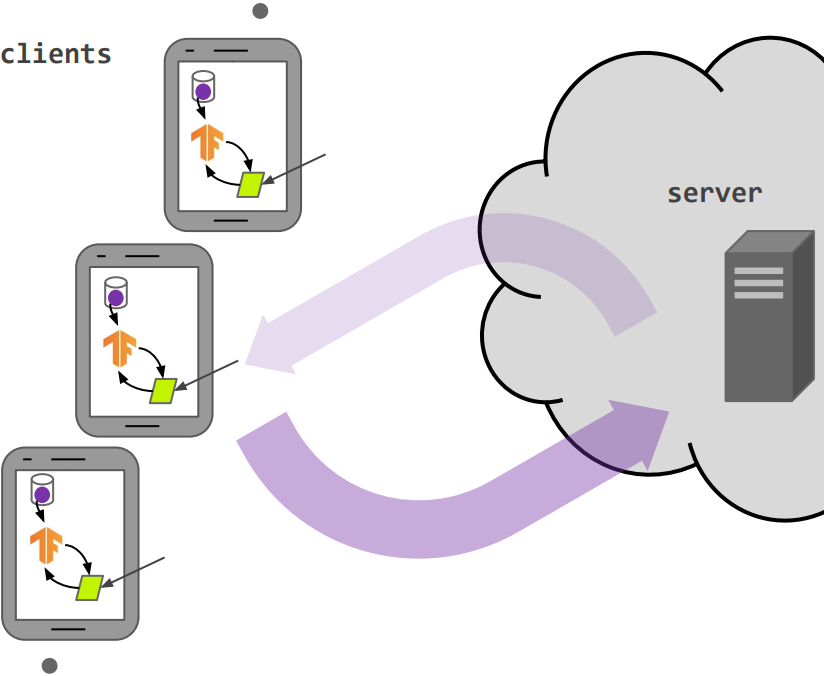
\includegraphics[width=0.7\textwidth]{Images/diagrams/FL_simplified.png}
        \decoRule
        \caption[FL system, simplified topology]{Simplified topology of an FL system \cite{survey_B}: \href{https://arxiv.org/abs/1912.04977}{URL}.}
        \label{fig: FL simplified topology}
\end{figure}

\section{Motivation}
Most FL research, to our knowledge, focuses on simulations and treats edge devices as black boxes; generally ignoring their nature and constrains. Taking in consideration the complexities of implementing ML on hardware, recent advancements in FL might be diminished or invalidated. The main motivation of this thesis is to identify, explore and possibly overcome the intrinsic conflicts that exist between FL and Artificial Neural Network (ANN) training in Field Programmable Gate Arrays (FPGA)s. % Such conflicts can be the batch size, where in FL tends to be minimized.

Instead of being incompatible, these two technologies may complement each other, which is worth investigating. Frequently in FL, transformations are applied on the generated ANN variables to reduce network utilization and enhance privacy. These transformations, which include quantization \cite{Mills2020}, adding Gaussian noise \cite{Wei2020} and others, tend to be spatially independent and could be implemented highly efficiently in hardware accelerators like FPGAs.

Finally, FL literature is almost devoid of wall-clock time examples. This thesis aims to provide a real world FL implementation that may be considered as a benchmark for future research. Furthermore, in order to be extendable and utilized in future works, the FL implementation is modular and platform independent.

\section{Scientific Contributions}
% The main focus of this thesis is combining FL training with FPGA based ANN implementations, while exploring and overcoming their inherent conflicts. Furthermore, it focus on the mostly unexplored FL setting of small client pools and its implicit difficulties. Finally, it provides a real world implementation of FL that can be used as a benchmark for future works. This FL implementation is agnostic of the ANN training implementation and can be used as a starting point for future works.
The main aim of this thesis is to explore the feasibility and efficiency of FL systems that employ FPGAs for the underlying training, focused on the edge setting. To achieve this, such a system was developed, thoroughly tested and benchmarked. Its components that can be utilized as starting points, examples or benchmarks of future works are as follows:
\begin{itemize}
    \item An FL system that is agnostic of the underlying ML model and training method. In the context of this work, it is employed with multiple ANNs of various types that are trained on CPU, GPU and FPGA. It can be easily modified to encompass other models and training implementations.
    \item A robustness analysis which focuses on the mostly unexplored FL setting of small client pools and its inherent difficulties.
    \item An FPGA-based implementation of training a CNN, that is optimized for the parameter space where the FL process is most efficient.
    \item Wall-clock timings of the CNN implementation and overall FL system, compared with equivalent implementations based on other technologies.
\end{itemize}
Finally, the aforementioned analyses and benchmarks are analyzed to provide apt suggestions for future works.

\section{Thesis Approach}
As the thesis moves forward, conflicts in terms of design and implementation are anticipated to arise between the two technologies. Furthermore, this is an mostly unexplored field. As such, a conservative and steady approach is expected to work best. 

Initially, a FL implementation that is agnostic and independent of the underlying training implementation, is developed. Its robustness is thoroughly validated, using TensorFlow to facilitate the local training. Subsequently, an FPGA-based CNN training implementation is created. 

Furthermore, an intermediate layer that connects the networking code of the FL clients with the FPGA driver is developed. With this approach, the FL implementation is combined with the FPGA-based implementation, and the overall system can be thoroughly tested and validated.

Finally, to benchmark the system, CPU and GPU implementation are developed and compared with it.

\section{Thesis Outline}
\begin{itemize}
    \item \textbf{Chapter 2 - Theoretical Background:} Description of the theoretical background of ML and FL.
    \item \textbf{Chapter 3 - Related Work:} Related works on FL, optimization techniques and hardware implementations of it.
    \item \textbf{Chapter 4 - FL architecture \& design:} Description of the FL architecture, design and implementation developed.
    \item \textbf{Chapter 5 - Robustness Analysis:} Analysis of the quality and performance of the FL implementation.
    \item \textbf{Chapter 6 - FPGA Implementation:} Description of the ANN architecture, design and implementation on FPGA developed.
    \item \textbf{Chapter 7 - Results:} Analysis of the quality and performance of the complete system. Comparisons with other technologies.
    \item \textbf{Chapter 8 - Conclusions and Related Work:} Conclusions and proposals for related future works.
\end{itemize}